\documentclass{beamer}

\usepackage{amsmath, amssymb}
\usepackage{tikz-cd}
\usepackage{xcolor}
\usepackage{graphicx}

\title{MAT222: Calculus II - Technique of Integration}
 \subtitle{7.8 Improper Integrals}

\author{\textbf{Miraj Samarakkody}}
\institute{Tougaloo College}
\date{Updated: \today}

\begin{document}

\begin{frame}
    \titlepage
\end{frame}


\begin{frame}{Introduction}
    
    \begin{block}{Definition}
        A \textbf{improper integral} is an integral that has one of the following properties:
        \begin{itemize}
            \item The interval of integration is infinite.
            \item The integrand is infinite at one or more points in the interval of integration.
        \end{itemize}
    \end{block}
\end{frame}

\begin{frame}{Type I - Infinite Intervals}
    Consider the infinite region \(S\) that lies under the curve \(y=1/x^2\), above the \(x-\)axis, and the right of the line \(x=1\). 

    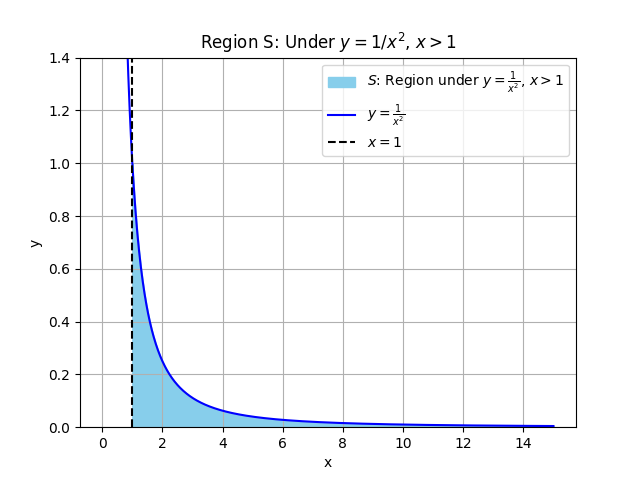
\includegraphics[scale=0.5]{figures/fig_2.png}
\end{frame}

\begin{frame}{Example}
    Evaluate the integral
    \[
        \int_1^\infty \frac{1}{x^2} \, dx
    \]
\end{frame}

\begin{frame}{Definition of an Improper Integral of Type I}
    \begin{itemize}
        \item If \(\int_{a}^{t}f(x)dx\) exists for every number \(t \geq a\), then \[\int_a^\infty f(x)dx = \lim_{t \to \infty} \int_a^t f(x) dx\] provided this limit exists. \pause
        \item If \(\int_{t}^{b}f(x)dx\) exists for every number \(t \leq b\), then \[\int_{-\infty}^b f(x)dx = \lim_{t \to -\infty} \int_t^b f(x) dx\] provided this limit exists. \pause
        \item The improper integrals \(\int_a^\infty f(x)dx\) and \(\int_{-\infty}^b f(x)dx\) are called \textbf{convergent} if the corresponding limits exists and are finite. Otherwise, they are called \textbf{divergent}.\pause
        \item If both \(\int_a^\infty f(x)dx\) and \(\int_{-\infty}^{a}f(x)dx\) are convergent, the we define \[
        \int_{-\infty}^{\infty} f(x)dx = \int_{-\infty}^{a}f(x)dx + \int_a^\infty f(x)dx    
        \]
    \end{itemize}
\end{frame}

\begin{frame}{Example}
    Determine whether the integral \(\int_1^\infty (1/x)dx\) is convergent or divergent. 
\end{frame}

\begin{frame}{Example 2}
    Evaluate \[\int_{-\infty}^0 x e^x~dx. \]
\end{frame}

\begin{frame}{Example 3}
    Evaluate \[\int_{-\infty}^{\infty}\dfrac{1}{1+x^2}dx\]
\end{frame}

\begin{frame}{Example 4}
    For what values of \(p\) is the integral \[\int_1^{\infty} \dfrac{1}{x^{p}}dx\] convergent? 
    
\end{frame}

\begin{frame}{Remark}
    \(\displaystyle \int_{1}^{\infty}\dfrac{1}{x^p}dx\) is convergent if \(p>1\) and divergent if \(p \leq 1\).
\end{frame}




\end{document}